\documentclass{SBCbookchapter}
\usepackage[utf8]{inputenc}
\usepackage[T1]{fontenc}
\usepackage[brazil,english]{babel}
\usepackage{graphicx}
\usepackage{booktabs}
\usepackage{amsmath,amssymb}

\author{Karla Geovanna Almeida de Sousa}
\title{NAP1 -- Projeto e Análise de Algoritmos:\\
       Primos, Tabela Hash e Busca em Grafos}

\begin{document}
\maketitle

\begin{center}
Bacharelado em Sistemas de Informação\\
Universidade Federal Rural da Amazônia (UFRA) -- Paragominas, PA, Brasil\\
\verb|karla.sousa@ufra.edu.br|
\end{center}

\begin{abstract}
This work experimentally compares three pairs of classical algorithms:
(i) brute-force primality testing versus Fermat's probabilistic test;
(ii) linear search versus hash-table search with chaining; and
(iii) breadth-first search (BFS) versus depth-first search (DFS) for
locating a target vertex in a graph. All experiments were implemented
in C and timed with \texttt{clock\_gettime(CLOCK\_MONOTONIC)}.
Results confirm the asymptotic analysis: brute force grows linearly
with $N$, whereas Fermat remains nearly constant; linear search grows
with $M$, whereas hashing keeps expected constant cost; BFS and DFS
share $O(V+E)$ complexity but exhibit different exploration and
memory profiles.
\end{abstract}

\begin{resumo}
\begin{otherlanguage}{brazil}
Este trabalho compara experimentalmente três pares de algoritmos
clássicos: (i) teste de primalidade por força bruta versus teste
probabilístico de Fermat; (ii) busca linear em vetor versus busca em
tabela hash com encadeamento; e (iii) busca em largura (BFS) versus
busca em profundidade (DFS) na localização de um vértice alvo em
grafos. Os experimentos foram implementados em linguagem~C e medidos
com \texttt{clock\_gettime(CLOCK\_MONOTONIC)}. Os resultados
confirmam a análise assintótica: a força bruta cresce linearmente com
$N$, enquanto Fermat é praticamente constante; a busca linear cresce
com $M$, enquanto a hash mantém custo esperado constante; BFS e DFS
têm a mesma complexidade $O(V+E)$, mas perfis de exploração e de
memória distintos.
\end{otherlanguage}
\end{resumo}

\section{Introdução}
A análise de algoritmos busca prever o custo de execução em função do
tamanho da entrada, mas a prática nem sempre acompanha a teoria:
constantes multiplicativas, localidade de memória e estrutura dos dados
alteram o desempenho real. Este relatório descreve três experimentos
independentes que confrontam pares de algoritmos com a mesma finalidade
e complexidades distintas, medindo tempos reais e comparando-os com a
previsão assintótica.

\section{Metodologia}
\label{sec:metodologia}
Todos os programas foram escritos em C (C11), compilados com
\texttt{gcc -O2 -Wall -Wextra -std=gnu11} e executados em Codespaces
Linux x86\_64 (container GitHub, 2 vCPUs, 8~GB RAM). Os tempos foram
medidos com \texttt{clock\_gettime(CLOCK\_MONOTONIC)}, com repetições
para reduzir ruído. Os dados brutos foram exportados em CSV e os
gráficos gerados com \texttt{matplotlib} (Python 3.11).

\subsection{Sub-atividade 1 --- Números primos}
Força bruta: testa todos os divisores $d \in \{2,\dots,n-1\}$. Fermat:
$k=10$ iterações com base $a \in [2,n-2]$ verificando
$a^{n-1} \equiv 1 \pmod{n}$ via exponenciação modular rápida
(\texttt{\_\_int128} para evitar overflow de 64 bits). Mediu-se o tempo
para primos crescentes (pior caso da força bruta): $7$, $101$,
$1\,009$, $10\,007$, $100\,003$, $1\,000\,003$, $10\,000\,019$,
$100\,000\,007$ e $1\,000\,000\,007$.

\subsection{Sub-atividade 2 --- Tabela hash}
Vetor de $M$ inteiros aleatórios em $[0,10M]$. Busca linear do início ao
fim. Tabela hash com encadeamento, tamanho = menor primo $\ge 2M$
($\alpha \approx 0{,}5$) e função multiplicativa de Knuth
$h(k) = (k \cdot 2654435761) \bmod \text{tam}$. Mediu-se o tempo médio
de busca por chave ausente (pior caso da linear) para
$M \in \{10^3, 10^4, 10^5, 10^6\}$.

\subsection{Sub-atividade 3 --- DFS e BFS}
Grafo não-dirigido conexo aleatório com $n=100\,000$ vértices e
$m=500\,000$ arestas (grau médio 10). BFS com fila circular; DFS com
pilha explícita. Ambos param ao encontrar o alvo. Mediu-se tempo e
vértices visitados, em média sobre $K=100$ alvos aleatórios.

\section{Resultados e Discussão}
\label{sec:resultados}

\subsection{Sub-atividade 1 --- Primalidade}
A Tabela~\ref{tab:primos} apresenta os tempos medidos.

\begin{table}[h!]
\caption{Tempos para primos crescentes ($k=10$).}
\label{tab:primos}
\begin{center}
\begin{tabular}{rccc}
\toprule
$N$ (primo) & Força bruta (s) & Fermat (s) & Razão FB/Fermat \\
\midrule
7             & $1{,}0\times10^{-7}$ & $4{,}1\times10^{-7}$ & 0{,}2 \\
101           & $2{,}4\times10^{-7}$ & $5{,}3\times10^{-7}$ & 0{,}5 \\
1 009         & $2{,}2\times10^{-6}$ & $8{,}2\times10^{-7}$ & 2{,}7 \\
10 007        & $2{,}2\times10^{-5}$ & $1{,}0\times10^{-6}$ & $2{,}1\times10^{1}$ \\
100 003       & $2{,}2\times10^{-4}$ & $1{,}3\times10^{-6}$ & $1{,}7\times10^{2}$ \\
1 000 003     & $2{,}3\times10^{-3}$ & $1{,}7\times10^{-6}$ & $1{,}4\times10^{3}$ \\
10 000 019    & $2{,}2\times10^{-2}$ & $2{,}8\times10^{-6}$ & $8{,}0\times10^{3}$ \\
100 000 007   & $2{,}2\times10^{-1}$ & $3{,}0\times10^{-6}$ & $7{,}3\times10^{4}$ \\
1 000 000 007 & $2{,}22$             & $3{,}6\times10^{-6}$ & $6{,}2\times10^{5}$ \\
\bottomrule
\end{tabular}
\end{center}
\end{table}

A Figura~\ref{fig:primos} (log-log) confirma a análise: a força bruta
cresce linearmente com $N$ (reta de inclinação 1), enquanto Fermat fica
praticamente horizontal. O cruzamento ocorre em torno de $N \approx
10^3$: abaixo, a força bruta é competitiva; acima, Fermat é ordens de
magnitude mais rápido. Para entradas pares, a força bruta é
$\Theta(1)$ e vence qualquer método probabilístico --- o melhor caso é
decisivo na escolha prática.

\begin{figure}[h!]
\centerline{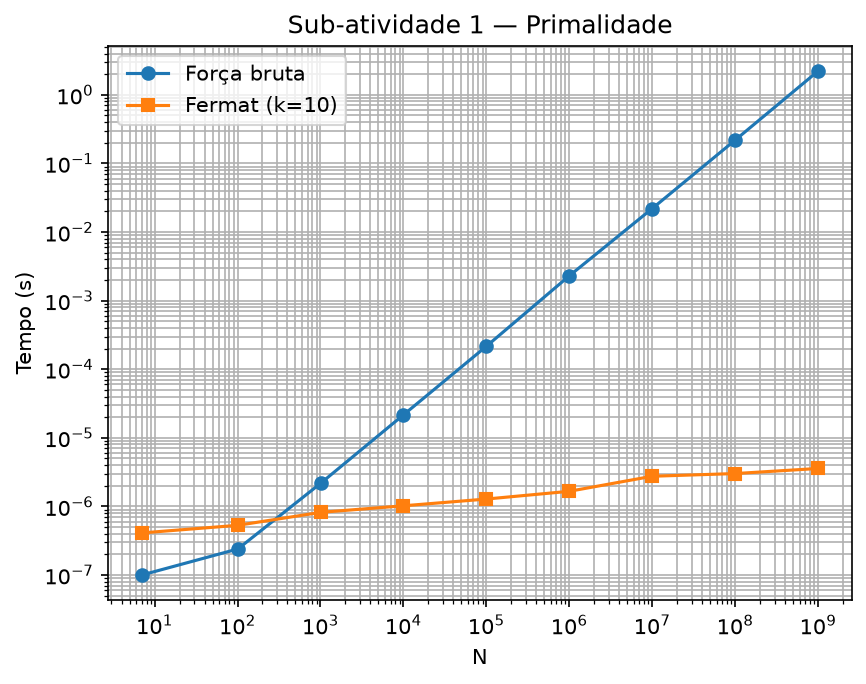
\includegraphics[width=0.75\linewidth]{../figures/fig_primos.png}}
\caption{Tempo de primalidade em função de $N$ (log-log).}
\label{fig:primos}
\end{figure}

\paragraph{Análise teórica.}
Força bruta: melhor caso $\Theta(1)$ (entrada par ou composto com fator
pequeno); pior caso $\Theta(n)$ (primo); complexidade $O(n)$. Fermat:
$O(k\log n)$; erro $\le 2^{-k}$ para compostos ímpares (Carmichael é
ressalva).

\subsection{Sub-atividade 2 --- Tabela hash}
A Tabela~\ref{tab:hash} mostra o tempo médio de busca por chave ausente.

\begin{table}[h!]
\caption{Tempo médio de busca (chave ausente).}
\label{tab:hash}
\begin{center}
\begin{tabular}{rccc}
\toprule
$M$ & Busca linear ($\mu$s) & Tabela hash ($\mu$s) & Aceleração \\
\midrule
$10^3$ & 0{,}41  & $<0{,}001$ & $4{,}3\times10^{2}$ \\
$10^4$ & 3{,}42  & $<0{,}001$ & $3{,}6\times10^{3}$ \\
$10^5$ & 33{,}74 & $0{,}003$  & $1{,}0\times10^{4}$ \\
$10^6$ & 350{,}63 & $0{,}006$ & $5{,}8\times10^{4}$ \\
\bottomrule
\end{tabular}
\end{center}
\end{table}

\begin{figure}[h!]
\centerline{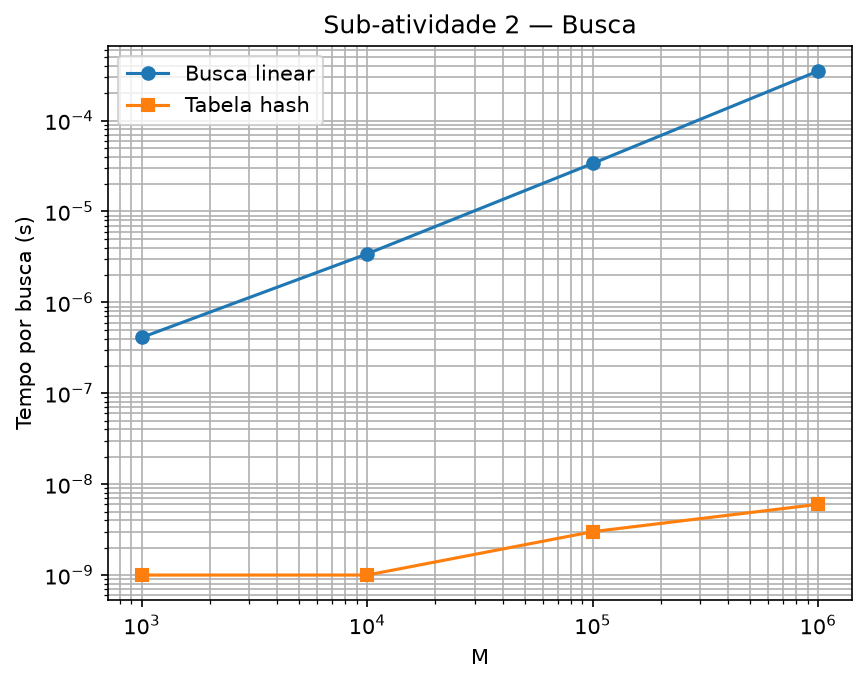
\includegraphics[width=0.75\linewidth]{../figures/fig_hash.png}}
\caption{Tempo de busca em função de $M$ (log-log).}
\label{fig:hash}
\end{figure}

A busca linear cresce linearmente com $M$ (reta de inclinação 1),
enquanto a hash permanece na ordem de poucos nanossegundos --- próxima
do limite de resolução do \texttt{clock\_gettime} ($\sim$~1~ns). Isso
confirma $\Theta(1+\alpha)$: com $\alpha \approx 0{,}5$, o custo
esperado é $O(1)$. O pior caso teórico da hash ($O(M)$, todas as chaves
no mesmo balde) não ocorre com função hash multiplicativa e tabela de
tamanho primo.

\paragraph{Análise teórica.}
Busca linear: melhor $\Theta(1)$ (chave na primeira posição), pior
$\Theta(M)$ (chave na última ou ausente), $O(M)$. Tabela hash: custo
esperado $\Theta(1+\alpha)$; com $\alpha \approx 0{,}5$, $O(1)$
esperado; pior caso $O(M)$; espaço $O(M+\text{tam})$.

\subsection{Sub-atividade 3 --- DFS e BFS}
A Tabela~\ref{tab:grafos} mostra a média sobre 100 alvos aleatórios.

\begin{table}[h!]
\caption{BFS versus DFS: $n=10^5$, $m=5\times10^5$, $K=100$ alvos.}
\label{tab:grafos}
\begin{center}
\begin{tabular}{lccr}
\toprule
Método & Tempo médio (ms) & Vértices visitados & Encontrou \\
\midrule
BFS & 11{,}14 & $50\,575$ & 100/100 \\
DFS & 12{,}75 & $50\,976$ & 100/100 \\
\bottomrule
\end{tabular}
\end{center}
\end{table}

\begin{figure}[h!]
\centerline{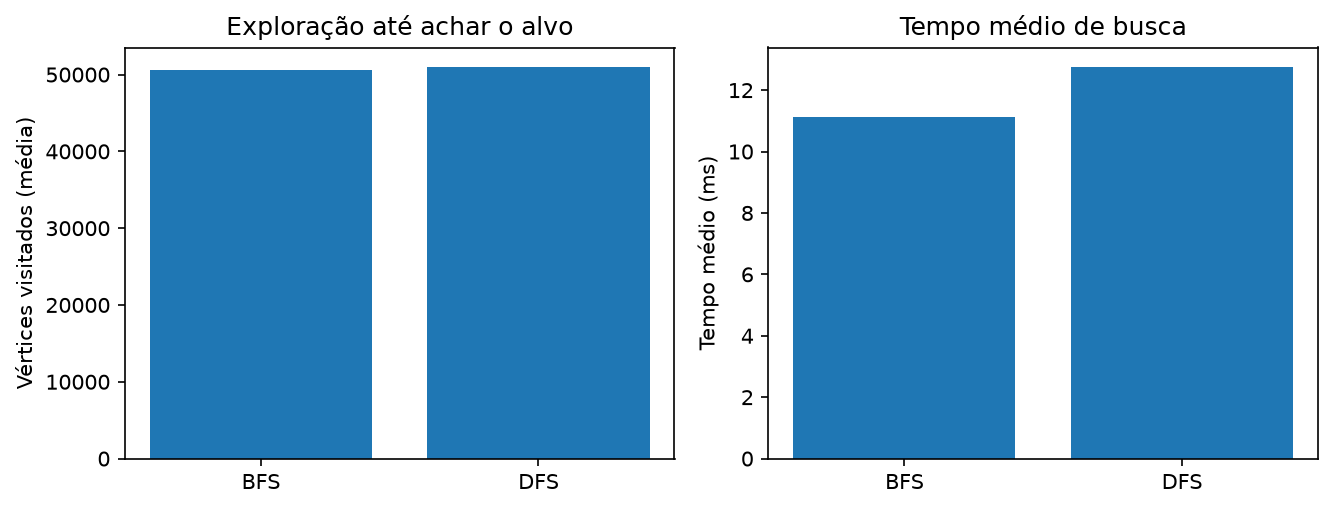
\includegraphics[width=0.75\linewidth]{../figures/fig_grafos.png}}
\caption{Vértices visitados e tempo médio até encontrar o alvo.}
\label{fig:grafos}
\end{figure}

Ambos visitaram aproximadamente metade dos $10^5$ vértices (50\,575 no
BFS e 50\,976 no DFS) e encontraram os 100 alvos. BFS foi ligeiramente
mais rápido (11,1~ms contra 12,8~ms, cerca de 13\% de vantagem), o que
se atribui à simplicidade do laço com fila circular e à boa localidade
de memória, além de o BFS visitar os vértices em ordem crescente de
distância. O fato de os dois métodos explorarem volumes parecidos de
vértices deve-se ao grau médio elevado do grafo aleatório
($\bar{d} = 10$): o diâmetro é pequeno frente a $n$, de modo que a
maior parte dos alvos está a poucos níveis da origem, mas o ``leque''
de vértices por nível cresce explosivamente --- em ambos os métodos, a
exploração acaba tocando quase toda a componente conexa. Em grafos
esparsos com estrutura de comunidade (redes sociais, malhas viárias), a
diferença costuma ser bem maior, com BFS visitando ordens de magnitude
menos vértices quando o alvo está próximo da origem.

\paragraph{Respostas às questões.}
\begin{enumerate}
  \item \textbf{Melhor/pior caso.} Melhor $O(1)$ quando o alvo é a
        origem (ou o primeiro vértice examinado); pior $O(V+E)$ quando
        o alvo está ausente ou é o último a ser descoberto. Em termos
        de memória, o pior caso do DFS é $O(V)$ (pilha) e o do BFS é
        $O(V)$ (fila), tipicamente maior em grafos largos.
  \item \textbf{Complexidade.} Com lista de adjacência, $O(V+E)$ para
        ambos. Com matriz de adjacência, $O(V^2)$.
  \item \textbf{Quando usar.} BFS: caminho mínimo em grafo não-ponderado,
        exploração por níveis, alvo próximo da origem. DFS: detecção
        de ciclos, ordenação topológica, componentes conexas e
        fortemente conexas, pontes e articulações, backtracking,
        grafos profundos com memória limitada.
\end{enumerate}

\section{Conclusão}
Os três experimentos confirmam a análise assintótica e mostram que a
escolha prática depende do contexto. (i) Para primalidade, a força
bruta só é vantajosa em entradas pequenas ou pares; Fermat é
indispensável para números grandes, chegando a $\sim$620 mil vezes de
aceleração em $N = 10^9$. (ii) A tabela hash troca espaço por tempo e
oferece ganho de 4 a 5 ordens de grandeza sobre a busca linear a
partir de $M \approx 10^4$. (iii) BFS e DFS têm a mesma complexidade
$O(V+E)$; em grafos aleatórios densos, como o testado, os dois
exploram volumes parecidos, mas BFS foi ligeiramente mais rápido. Em
grafos com estrutura mais realista, a diferença tende a ser maior.
Como trabalho futuro, sugere-se substituir Fermat por Miller--Rabin,
testar endereçamento aberto na hash e comparar DFS recursiva versus
iterativa.

\section{Referências}
\begin{thebibliography}{9}
\bibitem{cormen} CORMEN, T.~H. et al. \emph{Algoritmos: Teoria e
Prática}. 3.~ed. Rio de Janeiro: Elsevier, 2012.
\bibitem{ziviani} ZIVIANI, N. \emph{Projetos de Algoritmos com
Implementações em Java e C++}. São Paulo: Cengage, 2007.
\bibitem{sw} SEDGEWICK, R.; WAYNE, K. \emph{Algorithms}. 4.~ed.
Addison-Wesley, 2011.
\bibitem{knuth3} KNUTH, D.~E. \emph{The Art of Computer Programming,
Vol.~3}. 2.~ed. Addison-Wesley, 1998.
\bibitem{video1} Vídeo: DFS e BFS (geral).
\url{https://www.youtube.com/watch?v=MtlKYXC-sn8}.
\bibitem{video2} Vídeo: BFS (teoria).
\url{https://www.youtube.com/watch?v=b7guo8KcJ_w}.
\bibitem{video3} Vídeo: DFS (teoria).
\url{https://www.youtube.com/watch?v=gRYQAHAsXCI}.
\bibitem{video4} Vídeo: BFS em C.
\url{https://www.youtube.com/watch?v=qaCerM2qJ6l}.
\bibitem{video5} Vídeo: DFS em C.
\url{https://www.youtube.com/watch?v=v6DpcekKCb0}.
\end{thebibliography}

\end{document}
